\item O bloco deslizante $B$ está limitado a mover-se dentro da ranhura lisa. Ele está conectado a duas molas, cada uma com uma rigidez $k=\SI{30}{\newton/\meter}$. As molas estão originalmente estendidas \SI{.5}{\meter} quando $s=0$, como mostrado. Determine a distância máxima, $s_{\textit{máx}}$, que o bloco $B$ move-se após ser atingido pelo bloco $A$, que está originalmente movendo-se a $(v_{A})_{1}=\SI{8}{\meter/\second}$. Considere que $e=0.4$ e a massa de cada bloco seja \SI{1.5}{\kilogram}.

\begin{flushright}
	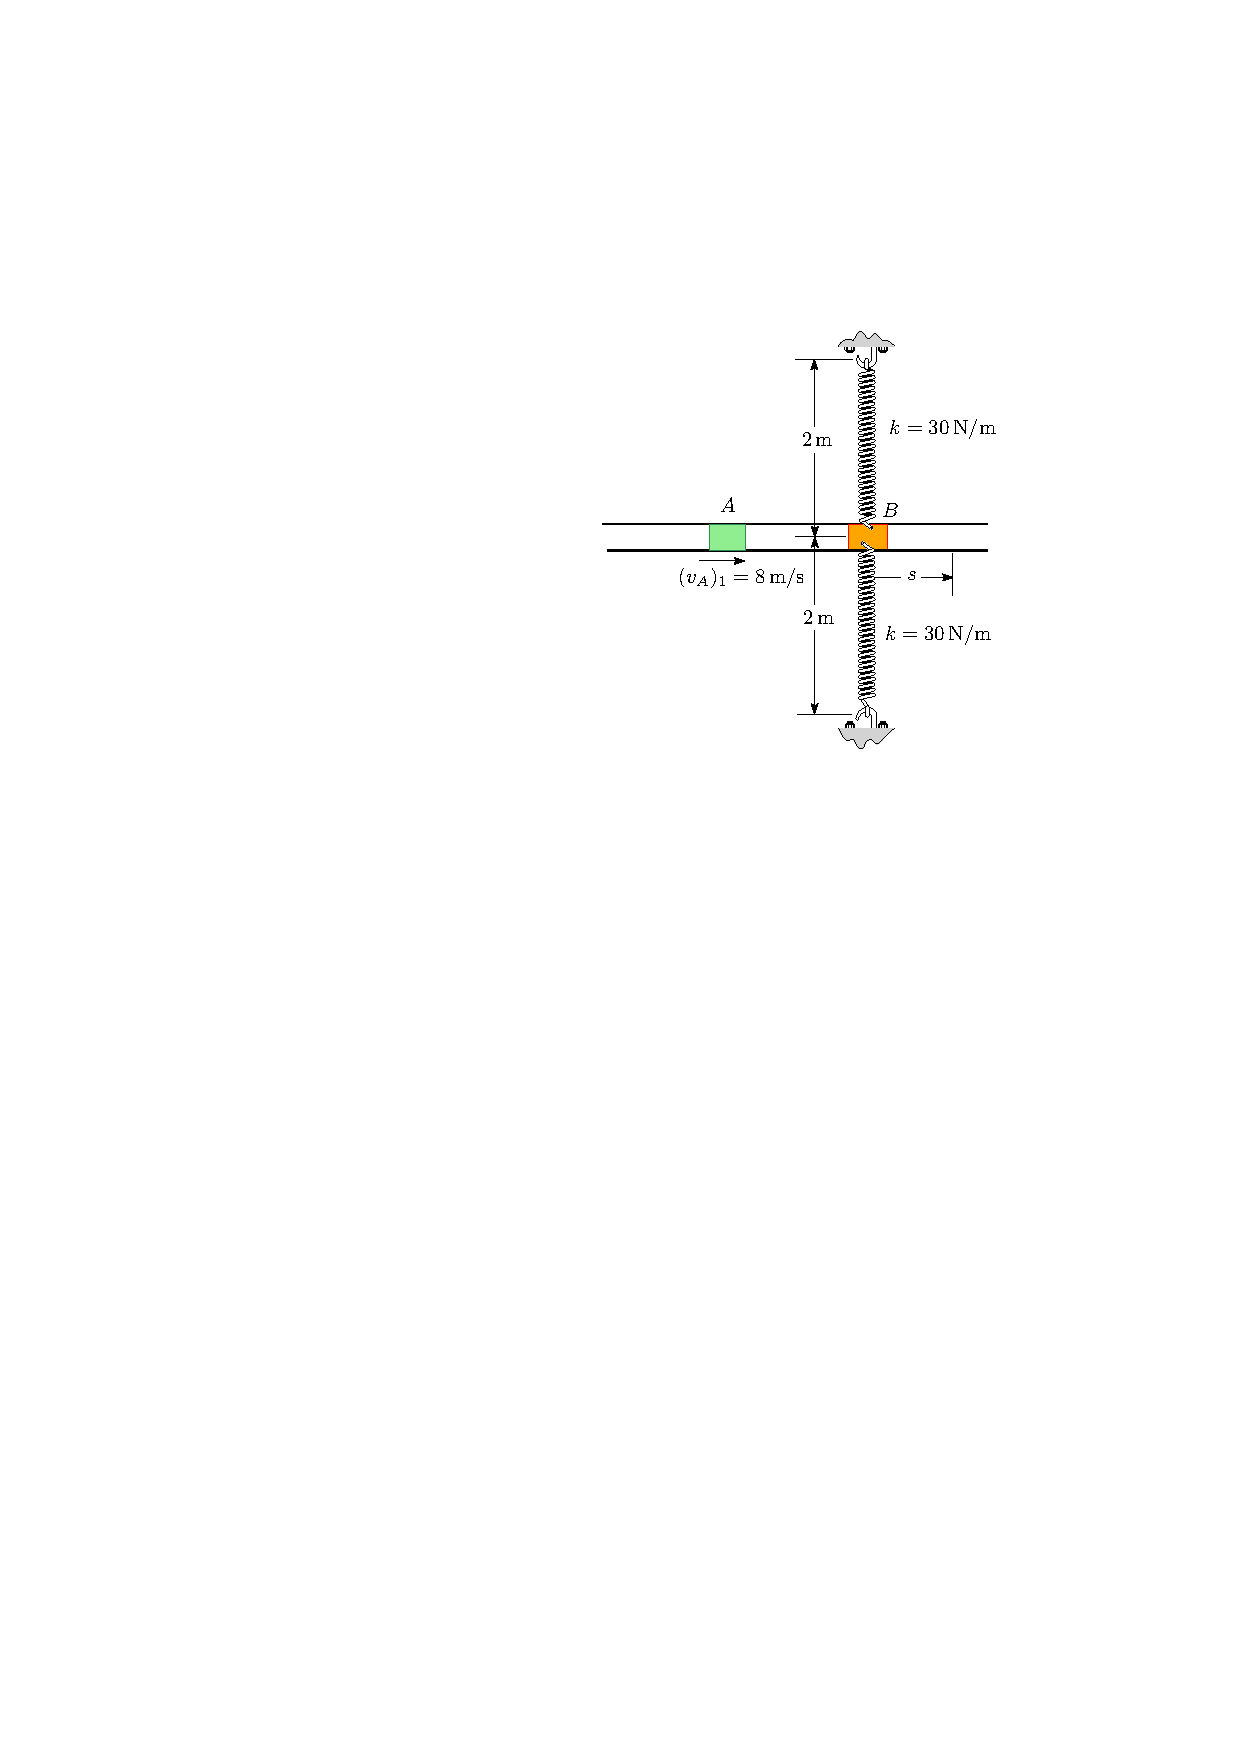
\includegraphics[scale=1.4]{images/draw_13}
\end{flushright}